Sistem tiket ini bergantung pada dua layanan lain, yaitu layanan pengguna dan pembayaran. Solusi yang berkomunikasi dengan layanan ini tidak boleh menjadi sumber \textit{bottleneck} agar hasil perbandingan berfokus pada \textit{bottleneck} dari sisi basis data.

\subsection{Layanan Pengguna}

Layanan ini tidak diimplementasikan dalam artian sebagai sebuah sistem yang menerima registrasi pengguna dan melayani \textit{login} pengguna. Proses registrasi dan \textit{login} dilakukan dari sisi \textit{virtual user} dengan membuat sendiri \textit{payload} JWT yang dikirim kes server agar prosesnya menjadi lebih cepat dari sisi latensi dan kebutuhan sumber daya. Apabila proses registrasi dan \textit{login} tetap dilakukan dari sisi server, maka layanan pengguna harus mampu melayani beban yang sama dengan sejumlah pengguna yang sedang diuji. Pendekatan ini tentu membutuhkan sumber daya komputasi yang cukup besar, tetapi tidak menambahkan nilai pada fokus yang ingin diuji pada penelitian ini.

\subsection{Layanan Pembayaran}

Layanan ini merupakan \textit{mock service} gerbang pembayaran. Layanan ini berpotensi menjadi sumber \textit{bottleneck} saat proses pembuatan tagihan, terlebih lagi karena komunikasi pembuatan tagihan harus dilakukan secara sinkron. Untuk memastikan \textit{throughput} yang tinggi, layanan ini akan menggunakan \textit{in-memory database} dengan \textit{persistence} seperti Redis. Redis akan dikonfigurasikan dalam mode kluster untuk kebutuhan \textit{sharding} dan \textit{multiple writer}. \textit{Persistence} dan \textit{snapshot} masih akan dikonfigurasikan, meski tetap akan ada periode waktu yang bisa mengakibatkan terjadinya \textit{data loss} (kurang dari satu detik). Skenario pengujian akan mengasumsikan tidak terjadinya kegagalan pada layanan ini, sehingga tidak ada data yang hilang.

Ketika pembayaran berhasil atau kadaluarsa, layanan ini akan memanggil \textit{webhook} pada layanan tiket. Untuk memastikan pemberitahuan terkirim, layanan ini akan melakukan \textit{retry} ketika terjadi kegagalan saat pemanggilan \textit{webhook}. Komponen \textit{timer} untuk \textit{expiration} dan \textit{queue} untuk pemanggilan \textit{webhook} juga akan menggunakan Redis.

Komponen pada layanan ini akan dibagi menjadi dua, yaitu \textit{payment processor} dan \textit{notifier}. \textit{Payment processor} merupakan komponen yang melayani pembuatan tagihan dan pembayaran tagihan. \textit{Notifier} merupakan komponen yang menangani \textit{timer} ketika terdapat pembayaran yang kadaluarsa dan  memanggil \textit{webhook} ketika pembayaran berhasil atau kadaluarsa. Setiap komponen dapat di-\textit{scale} secara horizontal.

\begin{figure}[htbp]
    \centering
    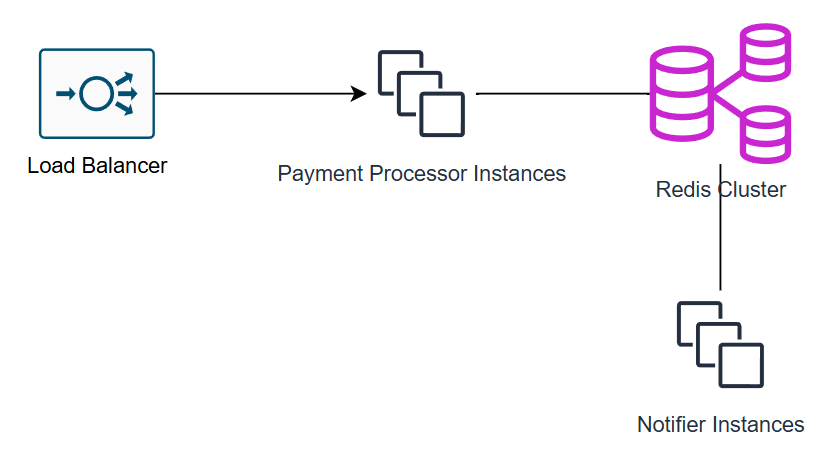
\includegraphics[width=0.8\textwidth]{resources/chapter-3/payment-service.png}
    \caption{Arsitektur Layanan Pembayaran}
    \label{fig:payment-service-deployment}
\end{figure}

Berikut adalah alur sistem pembayaran.

\begin{figure}[htbp]
    \centering
    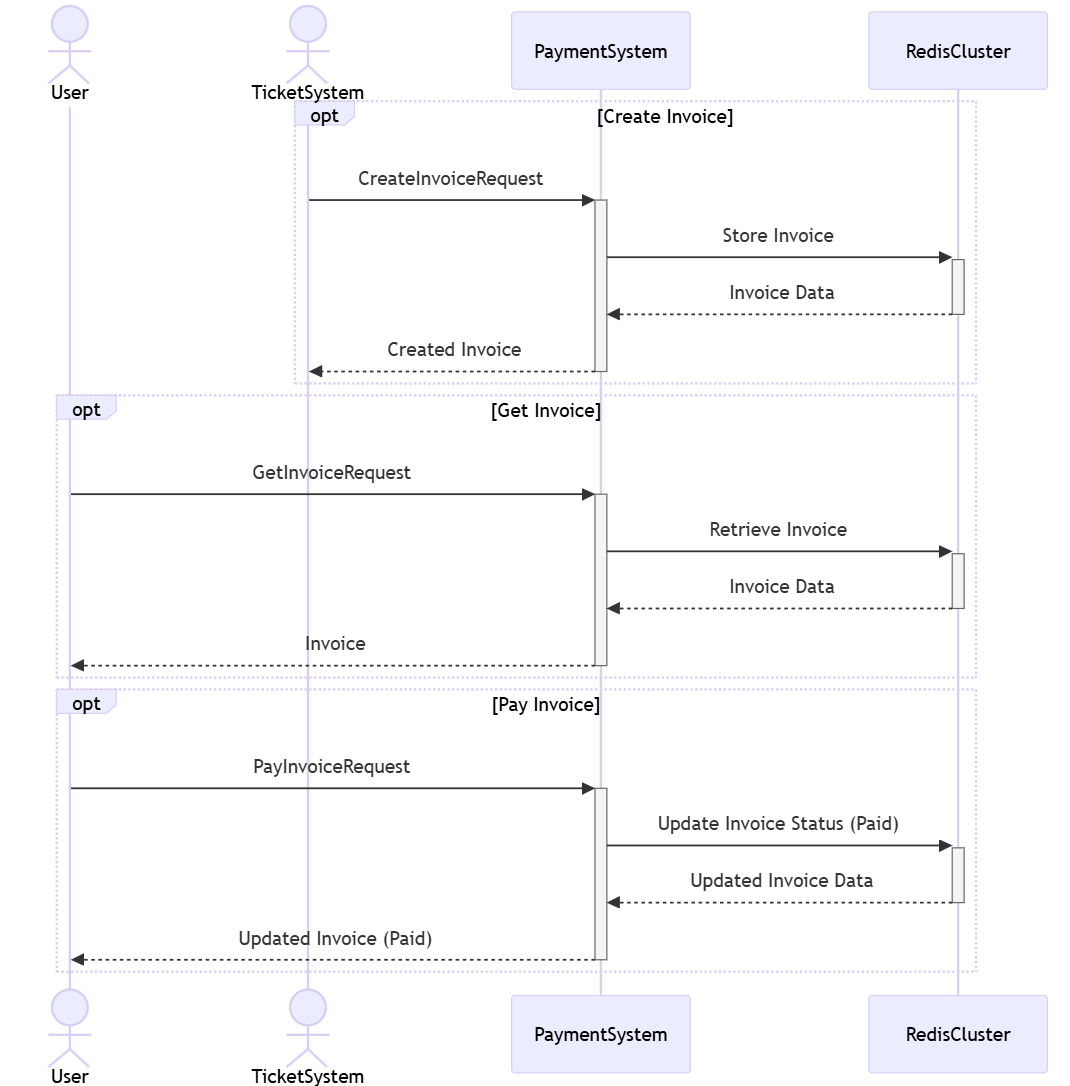
\includegraphics[width=0.8\textwidth]{resources/chapter-3/payment-flow1.png}
    \caption{Sequence Diagram 1 Layanan Pembayaran}
    \label{fig:payment-flow1}
\end{figure}

Sequence diagram di atas menunjukkan alur umum untuk operasi pembuatan Invoice, pembayaran Invoice, dan pengambilan data Invoice. Selanjutnya, sequence diagram di bawah menunjukkan alur untuk pemrosesan webhook untuk pembayaran pemesanan yang berhasil atau pun gagal. Skema webhook ini menggunakan strategi \textit{exponential backoff} untuk menangani kasus pemberitahuan yang gagal.

\pagebreak

\begin{figure}[htbp]
    \centering
    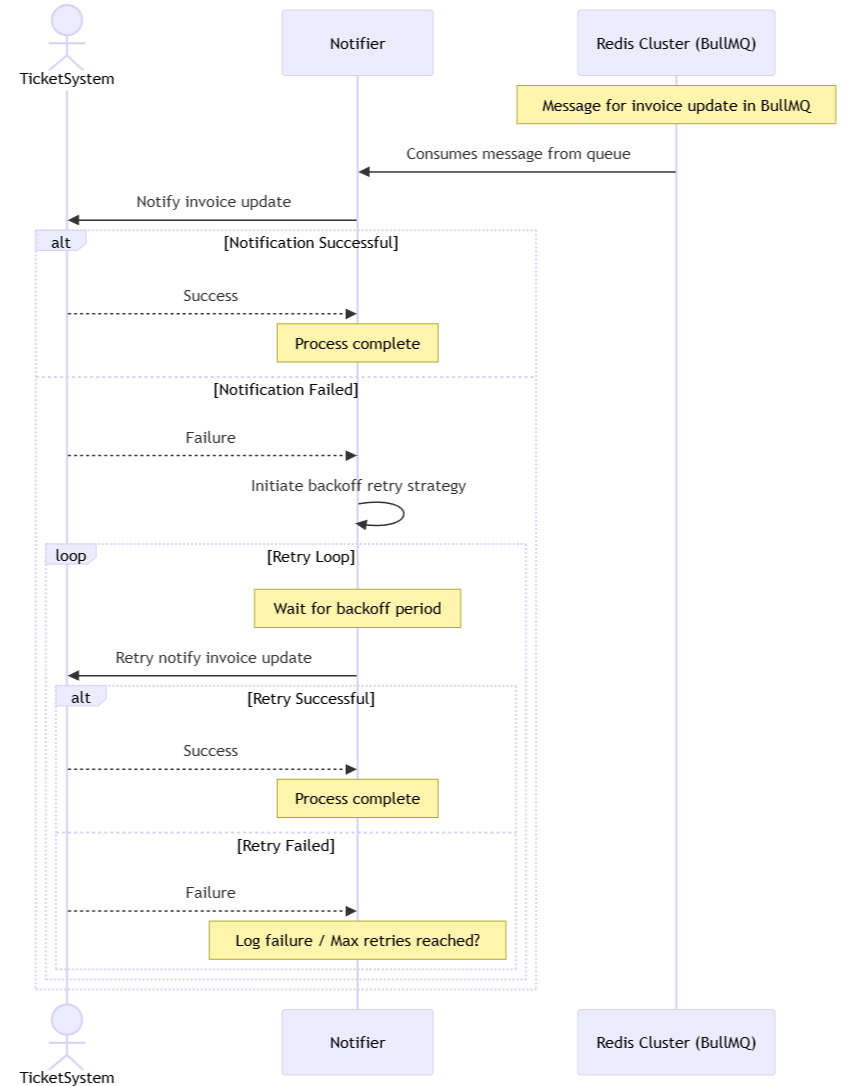
\includegraphics[width=0.8\textwidth]{resources/chapter-3/payment-flow2.png}
    \caption{Sequence Diagram 2 Layanan Pembayaran}
    \label{fig:payment-flow2}
\end{figure}